\chapter[PROCESSAMENTO DE DADOS]{PROCESSAMENTO DE DADOS}
\label{chapter:data}

A grande quantidade de geradores e consumidores de dados em cenários de cidades
inteligentes trazem a necessidade dos \textit{três V's} para as aplicações:
\textit{volume}, \textit{velocidade} e \textit{variedade} \cite{alnuaimi2015}.
Uma forma de atingir esses pontos é através do uso de tecnologias de
\textit{Big Data}, que podem ser utilizadas para armazenar, processar e analisar
os dados das aplicações de cidades inteligentes \cite{alnuaimi2015}. Como
relatado, o InterSCity carece de um serviço de processamento de dados mais
adequado, e a partir dos estudos que apresentamos neste capítulo, tomamos
decisões a respeito do novo serviço.

Levantamos duas arquiteturas: a Lambda, que é mais difundida, e a Kappa,
que escolhemos para utilização no novo serviço de processamento, e que é
uma resposta a arquitetura Lambda. Definimos também tecnologias que abranjam duas
formas de processamento: processamento em lote e processamento de fluxos.
No processamento em lote os dados são utilizados
em conjunto e armazenados de uma forma específica antes de serem escalonados
para o processamento \cite{zheng2015real}. No processamento
de fluxos, por outro lado, os dados são processados conforme estão
disponíveis \cite{zheng2015real}, permitindo consulta às informações com menor
latência. Descrevemos adaptações nas arquiteturas em relação ao apresentado
na literatura, com o propósito de maior adequação ao contexto de cidades
inteligentes e maior compatibilidade com os princípios e arquitetura de
microsserviços do InterSCity.

\section{ARQUITETURA LAMBDA}

A Arquitetura Lambda é um padrão de projeto para plataformas de processamento
de dados que utilizam tecnologias de \textit{Big Data} \cite{kiran2015}, e
surge como um caminho alternativo a outras arquiteturas mais antigas, como a
incremental com \textit{sharding} \cite{marz2015}. É composta de três camadas:
a camada \textit{batch}\footnote{No decorrer do texto, as camadas da
Arquitetura Lambda e outros termos associados não serão traduzidos.}, a camada
\textit{serving} e a camada \textit{speed} \cite{kiran2015}. Cada uma dessas
camadas é implementada utilizando algoritmos e ferramentas específicas, de modo
que certas ferramentas são mais apropriadas em certos contextos.

A \textbf{camada \textit{batch}} é responsável pelo processamento de uma grande
massa de dados, e tem como ponto fraco a alta latência. Em sua execução, ela
cria e gerencia um \textit{master dataset}\footnote{O \textit{master dataset} é um lote
histórico de informação, que, por ser imutável, só possibilita \textbf{anexação}
de informações.}, que após processado, tem seu resultado condensado em
visão de lotes, utilizados pela \textbf{camada \textit{serving}}.
A camada \textit{batch} é então, em sua essência, imutável, de modo que caso
uma mudança seja necessária, uma abordagem diferente deve ser seguida: o dado
que carece alteração não sofre transformações, permanecendo inalterado, mas um
novo dado com as alterações é inserido no lote \cite{marz2015}.

A \textbf{camada \textit{speed}} tem como diferencial o processamento com baixa
latência, que é obtido pelo uso de uma parcela menor da massa de dados\footnote{
A camada \textit{speed} só leva em conta dados que surgiram após a camada
\textit{batch} ter começado seu processamento.}. Outra característica importante
é que essa camada faz uso do processamento de fluxo de dados, estratégia que
processa os dados conforme ficam disponíveis. Esse tipo de
processamento funciona bem com mecanismos de passagem de mensagem
\cite{marz2015}, e permite que as consultas feitas levem em conta dados
recentes, ignorados temporariamente pela camada \textit{batch}. Por esses
motivos, a camada \textit{speed} também é conhecida como a camada que faz
\textit{processamento incremental} \cite{marz2015}, e que por aceitar a mutação
de dados, força o uso de um banco de dados que suporte escrita aleatória,
aumentando substancialmente a complexidade da solução \cite{marz2015}. Por
fim, a camada \textit{speed} condensa os resultados de seu processamento em
visões de tempo-real, que serão fundidos com os resultados das
visões de lote na apresentação do resultado final. Ao final, os resultados
da camada \textit{speed} são dispensados após um lote terminar seu
processamento \cite{marz2015}.

\begin{figure}[hbt]
  \centering
    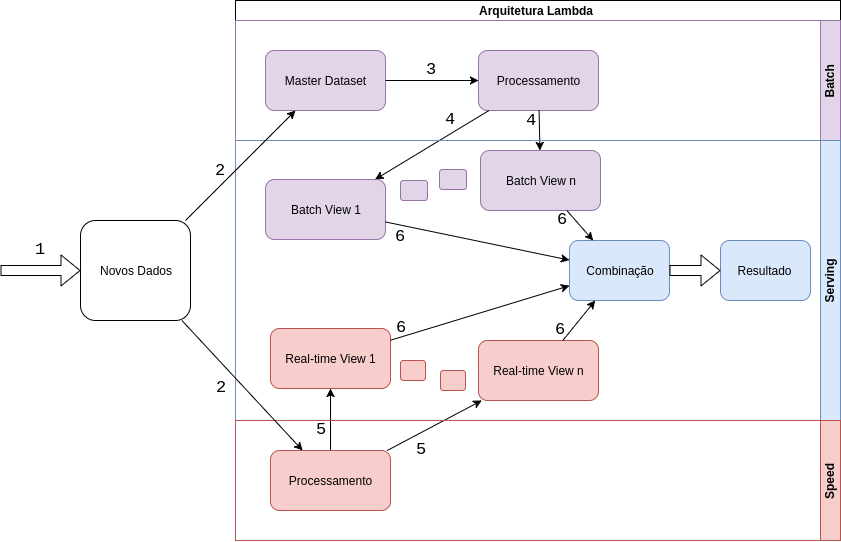
\includegraphics[width=\textwidth]{figuras/lambda-lifecycle.png}
    \caption{Ciclo de vida na Arquitetura Lambda. Baseado em: \citeonline{marz2015}.}
  \label{fig:lambda-lifecycle}
\end{figure}

Um ciclo de vida típico da Arquitetura Lambda pode ser acompanhado na Figura
\ref{fig:lambda-lifecycle}, e tem seu início com a (1) chegada
de novos dados, que são (2) transmitidos tanto para a camada
\textit{batch} quanto para a camada \textit{speed}. A camada \textit{batch}
(3) anexa os novos dados e os processa, (4) gerando assim
visão de lotes que são enviadas para a camada \textit{serving}. O mesmo
dado que foi enviado para a camada \textit{batch}, no passo (1), também foi
enviado para a camada \textit{speed}, onde (5) será processado com menor latência,
por só levar em conta dados recentes, gerando visões de tempo-real. 
Caso uma consulta seja feita ocorrerá uma (6) soma entre os resultados
dos visões de lote e visões de tempo-real, representando o resultado
desejado para a consulta \cite{marz2015}.

A Arquitetura Lambda garante sua resiliência através do \textit{isolamento de
complexidade}, que é obtido graças a separação entre camadas \textit{batch}
e \textit{speed} \cite{marz2015}. A resiliência é obtida pois, uma vez que os
resultados são processados na camada \textit{batch}, os resultados da camada
\textit{speed} podem ser descartados. Essa técnica é essencial, já que o
processamento em tempo-real pode criar inconsistências, por conta da baixa
precisão que é ocasionada por usar somente dados recentes; contudo, essa
inconsistência é corrigida no próximo lote a ser processado,
possibilitando que os resultados incoerentes da camada \textit{speed} sejam
descartados \cite{marz2015}.

Do ponto de vista da implementação no InterSCity, a Arquitetura Lambda pode
precisar de adaptações. Na literatura, a camada \textit{serving} é a responsável pela
junção entre o resultado do processamento feito pelas camadas \textit{speed} e
\textit{batch}, e a separação entre as camadas \textit{batch} e \textit{serving}
é bem definida \cite{marz2015}, contudo, isso depende das ferramentas
definidas para uso. 

\section{ARQUITETURA KAPPA}

A Arquitetura Kappa é um padrão de projeto de \textit{software}, e surgiu após
questionamentos\footnote{\url{https://www.oreilly.com/ideas/questioning-the-lambda-architecture}}
quanto a complexidade da Arquitetura Lambda. Kappa é uma arquitetura recente (2014) e
simples, e se baseia somente no uso da \textbf{camada \textit{speed}}
\cite{seyvet2016}. É guiada por quatro princípios: (1) tudo é um
fluxo de dados; (2) os dados devem ser imutáveis; (3) somente um
\textit{framework} para processamento deve ser utilizado; (4) os dados devem
armazenados, possibilitando a reprodução do estado \cite{seyvet2016}.

Fazendo uso da observação de que o \textit{log} é um conjunto de informações
imutáveis e com ordenação bem definida, a Arquitetura Kappa pode utilizá-lo
para atingir os quatro princípios citados anteriormente \cite{kreps2014}. O
\textit{log} é processado em tempo real, permitindo consultas em baixa
latência, com a possibilidade de acesso de dados atuais e históricos
\cite{forgeat2015}. Caso o processamento seja iniciado após o fluxo de dados já
ter começado, duas opções são possíveis: processar o \textit{log} do início,
tornando disponível os dados históricos; ou processar a partir do final,
não tendo acesso aos dados históricos, mas tendo latência mínima
\cite{kreps2014}.

\begin{figure}[hbt]
  \centering
    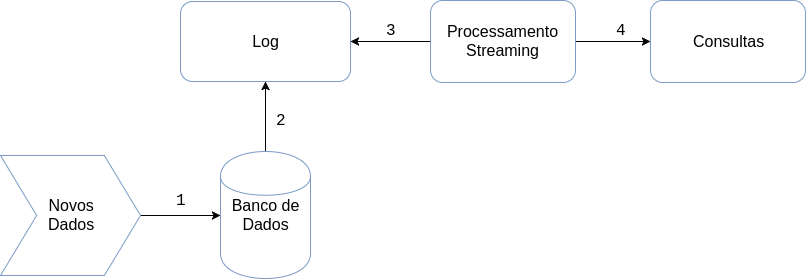
\includegraphics[scale=0.5]{figuras/kappa_architecture.png}
    \caption{Funcionamento da Arquitetura Kappa. Baseado em: \citeonline{seyvet2016}.}
  \label{fig:kappa-lifecycle}
\end{figure}

O funcionamento da Arquitetura Kappa está apresentado na Figura
\ref{fig:kappa-lifecycle}, e começa com a chegada de novos dados,
que são (1) publicados em tópicos do \textit{broker}. O \textit{broker} (2) anexa
os novos dados em um \textit{log} distribuído e (3) os transfere para
ferramentas de processamento em lote que estejam inscritas no tópico
relacionado. Por fim, (4) os resultados do processamento são disponibilizados
para serem consumidos.

Assim como levantado a respeito da Arquitetura Lambda, a implementação da
Arquitetura Kappa também pode precisar de adaptações para ser implantada no
InterSCity. Um casamento entre as tecnologias escolhidas deve ocorrer para que a
arquitetura seja implementada como sugerido na literatura, o que pode não ser
possível dadas as restrições da plataforma.

\section{BROKER}

A comunicação entre diferentes módulos em plataformas de processamento de dados
pode ocorrer de formas diversas, e no InterSCity é feita via passagem de
mensagem através do padrão PubSub \cite{delesposte2017}.
O \textbf{\textit{broker}} atua como mediador responsável por orquestrar as diferentes
mensagens que são transmitidas \cite{marz2015}, sendo primordial no
funcionamento das duas arquiteturas de \textit{Big Data} mencionadas anteriormente.

Uma abstração que facilita a compreensão do \textit{broker} é pensá-lo como o
mediador de um sistema de notícias. Uma entidade, desejando transmitir
uma notícia, a publica em um \textbf{tópico}, agindo como o produtor do
conteúdo. Outras entidades que desejam ser notificadas sobre aquele tema
inscrevem-se no tópico associado, e serão notificadas quando uma notícia referente
for publicada, agindo como consumidores. O \textit{broker} gerencia esse
processo, e tem a tarefa de transferir as mensagens de um emissor para
receptores.

\begin{figure}[hbt]
  \centering
    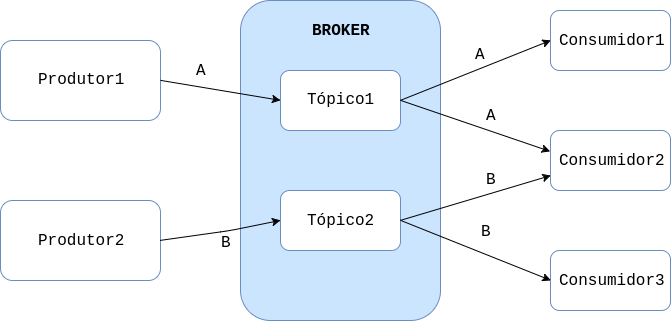
\includegraphics[scale=0.5]{figuras/broker.png}
    \caption{Funcionamento do \textit{broker}.}
  \label{fig:broker}
\end{figure}

A Figura \ref{fig:broker} ilustra o funcionamento do \textit{broker}, onde é
apresentado um cenário típico de atuação. No exemplo mostrado, a mensagem A
é transmitida pelo Produtor1 no Tópico1, e a mensagem B é transmitida pelo
Produtor2 no Tópico2. O Consumidor1 e o Consumidor2 recebem a mensagem A, por
estarem inscritos no Tópico1, e os consumidores Consumidor2 e Consumidor3
recebem a mensagem B, por estarem registrados no Tópico2. Esse funcionamento
pode receber variações, a depender das tecnologias utilizadas, e é útil
na implementação das arquiteturas Kappa e Lambda, sendo o
\textit{broker} o responsável por recuperar novas informações e as
disponibilizar para as ferramentas de processamento.

\section{COMPARATIVO ENTRE ARQUITETURAS}

De maneira geral, as duas opções (Kappa e Lambda) parecem funcionar bem em
cidades inteligentes. A Kappa pode ser vista como uma Arquitetura Lambda mais
simples, que se sustenta em um menor conjunto de ferramentas e
conceitos, enquanto a Lambda pode ser vista como uma opção segura,
capaz de lidar com quase todos os problemas do ecossistema de cidades
inteligentes. Decidimos pela Kappa, embora as duas arquiteturas apresentem
vantagens, sendo o contexto um dos fatores primordiais.

A Arquitetura Kappa, sem a reprodução dos dados, permite somente o uso de
algoritmos incrementais ou que não careçam analisar toda a massa de dados ao
mesmo tempo. Em um algoritmo de aprendizagem de máquina, por exemplo, a Kappa
pode funcionar, caso o treino do modelo seja incremental. Outro exemplo
seria o de filtros, como a busca por um termo específico dentro de um texto -
resultados anteriores não fazem diferença, e a Kappa mesmo sem a reprodução
dos dados resolveria bem. Contudo, caso seja desejado uma operação em toda
a massa de dados, como uma consulta em busca de um dado termo, a Kappa
não funciona, enquanto a Lambda pode escalonar um \textit{job} específico para essa
tarefa sem maiores problemas. Dessa forma, pela Lambda suportar algoritmos e tarefas
diferentes entre a camada \textit{batch} e a \textit{speed}, uma maior
flexibilidade fica disponível, o que pode ser importante para certos contextos.

\section{COMPARATIVO ENTRE TECNOLOGIAS}

Nesta seção apresentamos diferentes alternativas para compor a arquitetura do
novo serviço de processamentos do InterSCity. Separamos as ferramentas
nas categorias processamento em lote, processamento de fluxos
e \textit{broker}. Não analisamos ferramentas de banco de dados pois
uma troca seria prejudicial e não interessante para a equipe do InterSCity.
Analisamos um \textit{broker} diferente do utilizado pelo InterSCity,
considerando sua atuação somente com o serviço de processamento, não alterando
os microsserviços existentes da plataforma.

\subsection{Ferramentas de Processamento Batch}

Analisamos duas ferramentas de processamento em lote: o \textbf{Apache
Hadoop MapReduce}, precursor no ecossistema \textit{Big Data}, e o
\textbf{Apache Spark}, que optamos para compor o novo serviço de processamento.
O Hadoop MapReduce é uma das ferramentas que compõe o ecossistema do Hadoop, e
já foi utilizado, com excelência, em cenários de grande massa de
dados\footnote{Lista das empresas que utilizam ou já utilizaram o Hadoop:
\url{https://wiki.apache.org/hadoop/PoweredBy}} \cite{zaharia2008}.
Dispõe apenas de API nativa para linguagem Java, de modo que o uso do Hadoop
MapReduce no InterSCity deva utilizar a saída e entrada padrão do
Sistema Operacional para que seja possível o desenvolvimento em Ruby, linguagem
de maior domínio pelo time do InterSCity.

Um dos questionamentos feitos ao Hadoop MapReduce é em relação ao constante acesso e
uso do disco, que deve ser feito sempre que um \textit{job} é finalizado. Por
conta dessa característica, seu uso não é facilmente justificável em cenários em
que a massa de dados não é grande o suficiente, e uma opção válida acaba sendo
o Apache Spark, que troca o uso do disco pelo uso da memória, através da estratégia
de micro-lotes \cite{arsalan2014}. Os micro-lotes têm tempo de processamento
definidos em código, de modo que seja possível definir tempos de
micro-lotes pequenos o suficiente para que seja considerado
tempo-real\footnote{O tempo-real mencionado é sempre o \textit{soft real-time}.}.

\begin{table}[!htbp]
    \centering
    \caption[Resultados da Sort Benchmark 2014, categoria GraySort]{Resultados da Sort Benchmark 2014, categoria GraySort. Fonte: Databricks, 2014\footnotemark.}
    \label{tab:graysort2014results}
    \resizebox{\textwidth}{!}{%
        \begin{tabular}{|l|l|l|l|}
            \hline
             & \textbf{Hadoop MRRecord}      & \textbf{SparkRecord}             & \textbf{Spark1 PB}               \\ \hline
             Data Size                    & 102.5 TB                      & 100 TB                           & 1000 TB                          \\ \hline
             Elapsed Time                 & 72 mins                       & 23 mins                          & 234 mins                         \\ \hline
             \# Nodes                     & 2100                          & 206                              & 190                              \\ \hline
             \# Cores                     & 50400 physical                & 6592 virtualized                 & 6080 virtualized                 \\ \hline
             Cluster disk throughput      & 3150 GB/s(est.)               & 618 GB/s                         & 570 GB/s                         \\ \hline
             Sort Benchmark Daytona Rules & Yes                           & Yes                              & No                               \\ \hline
             Network                      & dedicated data center, 10Gbps & virtualized (EC2) 10Gbps network & virtualized (EC2) 10Gbps network \\ \hline
             \textbf{Sort rate}           & \textbf{1.42 TB/min}          & \textbf{4.27 TB/min}             & \textbf{4.27 TB/min}             \\ \hline
             \textbf{Sort rate/node}      & \textbf{0.67 GB/min}          & \textbf{20.7 GB/min}             & \textbf{22.5 GB/min}             \\ \hline
        \end{tabular}
    }
\end{table}

Outras características importantes do Spark para o contexto do
InterSCity são: API nativa em Python, Scala, Java e R; biblioteca de
processamento de fluxos, permitindo que o Spark seja utilizado também na camada
\textit{speed} da Arquitetura Lambda; e biblioteca de clusterização e
aprendizagem de máquina, que pode ser útil para compor o futuro canal de
processamento de dados do InterSCity. A Tabela \ref{tab:graysort2014results}
apresenta um comparativo entre o desempenho do Hadoop MapReduce e do Spark, pela
competição SortBenchmark\footnote{\url{http://sortbenchmark.org/}}. Na
competição, o Spark apresentou um desempenho três vezes maior que o Hadoop
MapReduce, utilizando dez vezes menos recursos.

\footnotetext{\url{https://databricks.com/blog/2014/11/05/spark-officially-sets-a-new-record-in-large-scale-sorting.html}}

\subsection{Ferramentas de Processamento de Fluxos}

Analisamos duas ferramentas de processamento de fluxos: O
\textbf{Apache Storm}, escrito por Nathan Marz, criador da Arquitetura
Lambda, e o \textbf{Apache Spark}, analisado anteriormente como ferramenta de
processamento em lote, e que escolhemos para uso no novo serviço de
processamento. O Apache Storm permite o uso de qualquer
linguagem de programação que interaja com a saída e entrada padrão do Sistema
Operacional, e sendo sugerido por Nathan Marz em seu livro sobre a Arquitetura
Lambda \cite{marz2015}, se faz uma opção segura para compor a camada
\textit{speed}.

O Spark é utilizado como ferramenta de processamento de fluxos graças ao seu módulo
Spark Streaming, que tem nativamente integração com outras ferramentas que
podem servir de produtores, como o Kinesis, Kafka, HDFS, dentre outras. O
grande diferencial entre o Spark e o Storm é que o Spark faz processamento
de fluxos via micro-lotes, ou seja, processa em intervalo
de tempos pré-definidos, enquanto o Storm processa em tempo-real, conforme
chegam novos dados. Essa diferença resulta em um tempo de latência notável
entre os dois, onde o Spark apresenta tempo de latência com pouca variância
conforme o volume de dados aumenta, enquanto o Storm apresenta latência mínima
com baixo volume de dados, mas que vai aumentando conforme o volume aumenta.
Um estudo feito relatou a diferença de desempenho entre as duas
ferramentas\footnote{\url{http://xinhstechblog.blogspot.com.br/2014/06/storm-vs-spark-streaming-side-by-side.html}},
contudo, o cenário aplicado utilizava pequena massa de dados, favorável ao
Storm.

O Storm apresenta como vantagem em relação ao Spark o desempenho
superior e a flexibilidade de uso da linguagem Ruby, já utilizada pelo time
do InterSCity, porém o Spark conta com a possibilidade de processamento
em lote, integração nativa com ferramentas produtoras e o acesso a
ferramentas de clusterização e aprendizagem de máquina, que por serem
interessantes para o InterSCity, equilibram o \textit{trade-off} entre as
duas ferramentas.

\subsection{Broker}

Analisamos dois \textit{brokers}: o \textbf{RabbitMQ}, utilizado
extensivamente pelo InterSCity, e o \textbf{Apache Kafka}, constantemente
referenciado para implantação da Arquitetura Kappa. O RabbitMQ é um
\textit{broker} bem difundido, utilizado por empresas como a Cisco, Instagram,
New York Times, dentre outros\footnote{\url{https://www.rabbitmq.com/}},
e apresenta suporte para diversas linguagens \cite{zaitsev2014}, o que
facilitou sua adoção pelo time do InterSCity. Podem ser destacados como
diferenciais do RabbitMQ em relação a outros \textit{brokers}: tolerância a
falhas, processamento distribuído, alto desempenho, filas (e tópicos) com
composições mais complexas e a possibilidade de uso de
\textit{plugins}\footnote{\url{https://www.rabbitmq.com/plugins.html}},
que suportam, por exemplo,
federação\footnote{\url{https://www.rabbitmq.com/federation.html}}.

O Apache Kafka, que foi a ferramenta que decidimos para compor o novo serviço,
é uma ferramenta mais nova\footnote{O RabbitMQ teve
sua primeira versão estável em 2007, e o Apache Kafka em 2011.}, e também é
utilizado em produção por diversas
empresas\footnote{\url{https://cwiki.apache.org/confluence/display/KAFKA/Powered+By}}.
Tendo como principais diferenciais o desempenho e a escalabilidade,
recentemente foi capaz de lidar com mais de 1.4 trilhões de mensagens diárias,
distribuídas sobre 1400 nós \cite{koshy2016}. Um outro diferencial relevante
entre o Kafka e os outros concorrentes é o suporte padrão a integração entre
\textit{logs} e tópicos, importante na implementação da Arquitetura Kappa. Ainda,
o Kafka conta com sistema de tolerância a falhas e suporte a várias linguagens de
programação\footnote{\url{https://cwiki.apache.org/confluence/display/KAFKA/Clients}}.

Ambas as opções são sólidas e adequadas para o uso do InterSCity. O
desempenho entre os dois já foi comparado, e embora o Kafka tenha tido desempenho
superior\footnote{\url{http://www.cloudhack.in/2016/02/29/apache-kafka-vs-rabbitmq/}},
o desempenho do RabbitMQ não compromete o uso no InterSCity. Assim, os pontos
cruciais que levamos em conta na escolha de tecnologia foram: o fato do Kafka
ter suporte a \textit{log} e \textit{handler} nativo para o Spark, e o RabbitMQ
já ser utilizado pelo InterSCity e ter o uso estendido via \textit{plugins}.
Assim, a escolha por qualquer uma dentre as duas tecnologias parece certa, mas
ao final optamos pelo Kafka, pelos pontos citados.
